% F8 — Two harnesses: the runtime harness that walks a burst (left) and the evaluation harness that judges a change
% to it (right). Single-column figure (~3.3 in). COLOUR GRAMMAR (decisions 24/26): blue = code, green = model role,
% white = documents/records, amber = human, dashed = PROPOSED; Source Sans Pro; 1 pt soft-grey round arrows.
% Counts (census 2026-09-03): 134 tests in 11 files; 25 promoted tables audited; EVAL_<utc>.json carries
% model_id + git_head (dev/eval_battery.sh). Known-results replay = PROPOSED (roster row 41 / T1).
\documentclass[tikz,border=4pt]{standalone}
\usepackage[T1]{fontenc}
\usepackage[default]{sourcesanspro}
\usetikzlibrary{positioning,fit,calc,shapes.geometric,arrows.meta,backgrounds}
\newcommand{\nohyph}{\hyphenpenalty=10000 \exhyphenpenalty=10000 }
\definecolor{codefill}{RGB}{199,217,239}\definecolor{codeline}{RGB}{59,110,165}
\definecolor{agentfill}{RGB}{226,240,217}\definecolor{agentline}{RGB}{58,125,52}
\definecolor{humanfill}{RGB}{253,236,200}\definecolor{humanline}{RGB}{191,124,0}
\begin{document}
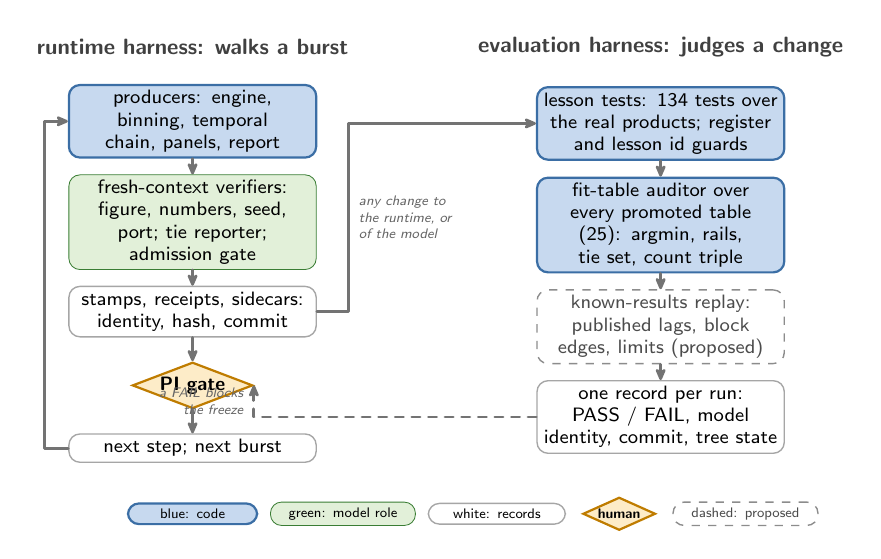
\begin{tikzpicture}[
  font=\sffamily\scriptsize, node distance=2mm and 3mm,
  box/.style={draw=black!35, line width=0.5pt, rounded corners=4pt, fill=white, text width=30mm, align=center, inner sep=2pt, execute at begin node=\nohyph},
  code/.style={box, fill=codefill, draw=codeline, line width=0.8pt},
  agent/.style={box, fill=agentfill, draw=agentline, line width=0.3pt},
  prop/.style={box, dashed, draw=black!45, text=black!70},
  human/.style={draw=humanline, thick, diamond, aspect=2.6, fill=humanfill, inner sep=0.5pt, font=\sffamily\scriptsize\bfseries},
  head/.style={font=\sffamily\footnotesize\bfseries, text=black!75},
  arr/.style={-{Stealth[length=2mm,width=1.7mm,round]}, line width=1pt, black!55, line cap=round, line join=round},
  lab/.style={font=\sffamily\tiny\itshape, text=black!60, execute at begin node=\nohyph}]

% left column: runtime harness
\node[head] (hl) {runtime harness: walks a burst};
\node[code, below=2.5mm of hl] (prod) {producers: engine, binning, temporal chain, panels, report};
\node[agent, below=of prod] (ver) {fresh-context verifiers: figure, numbers, seed, port; tie reporter; admission gate};
\node[box, below=of ver] (stamp) {stamps, receipts, sidecars: identity, hash, commit};
\node[human, below=3mm of stamp] (gate) {PI gate};
\node[box, below=3mm of gate] (next) {next step; next burst};
\draw[arr] (prod) -- (ver); \draw[arr] (ver) -- (stamp); \draw[arr] (stamp) -- (gate); \draw[arr] (gate) -- (next);
\draw[arr] (next.west) -- ++(-3mm,0) |- (prod.west);

% right column: evaluation harness
\node[head, right=14mm of hl] (hr) {evaluation harness: judges a change};
\node[code, below=2.5mm of hr] (tests) {lesson tests: 134 tests over the real products; register and lesson id guards};
\node[code, below=of tests] (audit) {fit-table auditor over every promoted table (25): argmin, rails, tie set, count triple};
\node[prop, below=of audit] (known) {known-results replay: published lags, block edges, limits (proposed)};
\node[box, below=of known] (rec) {one record per run: PASS / FAIL, model identity, commit, tree state};
\draw[arr] (tests) -- (audit); \draw[arr] (audit) -- (known); \draw[arr] (known) -- (rec);

% the coupling
\draw[arr] (stamp.east) -- ++(4mm,0) |- node[lab, pos=0.25, right, text width=13mm, align=left] {any change to the runtime, or of the model} (tests.west);
\draw[arr, dashed] (rec.west) -| node[lab, pos=0.75, left, text width=12mm, align=right] {a FAIL blocks the freeze} (gate.east);

% legend
\node[code, below=5mm of next, text width=15mm, font=\sffamily\tiny] (l1) {blue: code};
\node[agent, right=1.5mm of l1, text width=17mm, font=\sffamily\tiny] (l2) {green: model role};
\node[box, right=1.5mm of l2, text width=16mm, font=\sffamily\tiny] (l3) {white: records};
\node[human, right=2mm of l3, aspect=2.2, font=\sffamily\tiny\bfseries] (l4) {human};
\node[prop, right=2mm of l4, text width=17mm, font=\sffamily\tiny] (l5) {dashed: proposed};
\end{tikzpicture}
\end{document}
